\documentclass{IEEEtran}
\usepackage[utf8]{inputenc}
\usepackage[alsoload=synchem,load=named]{siunitx}
\usepackage[version=4]{mhchem}
\usepackage{amsmath}
\usepackage{graphicx}

\graphicspath{{images/}}

\let\DeclareUSUnit\DeclareSIUnit
\let\US\SI
\DeclareUSUnit\foot{ft}
\DeclareUSUnit\inch{in}

\author{Powers-Luhn, J.R.}
\title{Neural Network Overfitting in Non-linear Systems}
\date{June 20th, 2017}

\begin{document}
\maketitle

\section{Introduction}
The development of predictive models depends on fitting training data to sufficient accuracy, while not sacrificing the general nature of these models. In the case of non-linear neural networks, this presents a challenge as the convergence of the model is stochastic in nature. Further, network training depends on the selection of training method and parameters, as well as the initial parameters of the network. In order to demonstrate this, a single-layer neural network was trained on a well-characterized (no noise) data set in order to examine the effects of varying the number of hidden neurons on overfitting training data.

\section{Methods}
A set of training data was generated with the nonlinear function $y = 0.1 x_1 + 3 x_2 - x_1 x_2 $. A neural network was created using the matlab \verb|feedforwardnet| function with the ability to adjust the number of neurons in the hidden network programatically. An example diagram is shown in figure \ref{fig:example_network}. The network was configured to minimize the sum of the squared errors, seeking a target of 1 or below. Training data was generated with $x_1$ and $x_2$ in the range of $\left[0, 1, ..., 10 \right]$, normalized to zero mean and unit variance. A \verb|logsig| function was used as the activation function in the hidden layer, with a linear function in the output layer.

\begin{centering}
\begin{figure}
\begin{center}
	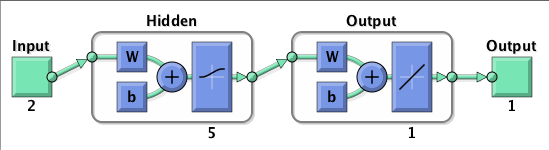
\includegraphics[width=0.4\textwidth]{network}
	\caption{Example of network design employed\label{fig:example_network}}
\end{center}
\end{figure}
\end{centering}

In order to test the efficacy of the trained network within the bounds of the training data, the interval between the independent variable was changed from 1 to 0.1. The network was evaluated at each of these points and the results compared to the calculated values. A similar procedure was performed to evaluate the network outside of the training domain with the independent variable ranging from $\left[-5,15\right]$ in units of 0.1.

\section{Results}
It was determined that the minimum number of nodes to train the network was two, as shown in figure \ref{fig:trainperf}. Above this value no additional reduction in training time was observed (of note, the network training stopped when the SSE for the training set was reduced below one).

\begin{centering}
\begin{figure}
\begin{center}
	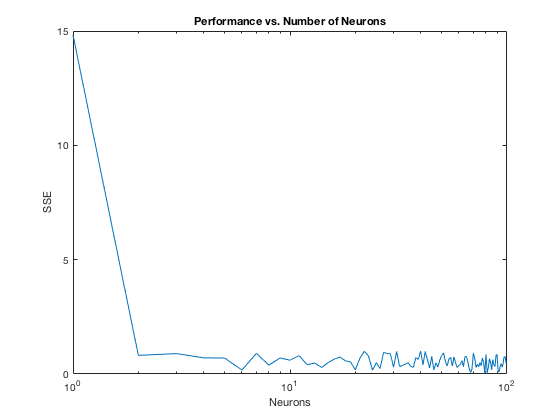
\includegraphics[width=0.4\textwidth]{fit_vs_neurons}
	\caption{Network error vs. Hidden Neurons\label{fig:trainperf}}
\end{center}
\end{figure}
\end{centering}

The network showed unexpected variation within the dataset, with error increasing as the input magnitude increased within the training range, as shown in figure \ref{fig:interp_error}.

\begin{centering}
\begin{figure}
\begin{center}
	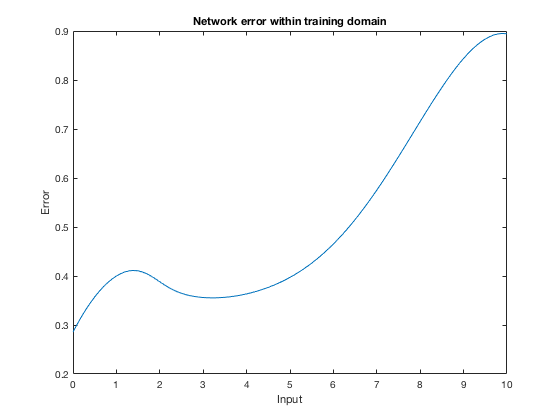
\includegraphics[width=0.4\textwidth]{interp_error}
	\caption{Interpolation error (in units of $\sigma$) \label{fig:interp_error}}
\end{center}
\end{figure}
\end{centering}

Outside of the dataset the network showed a maximum error in at approximately [12, 12], with error decreasing at higher input values in the range evaluated, as seen in figure \ref{fig:extrap_error}. Below the training range error did not extend past $-0.5\sigma$, though the slope indicated increasing magnitude of error.

\begin{centering}
\begin{figure}
\begin{center}
	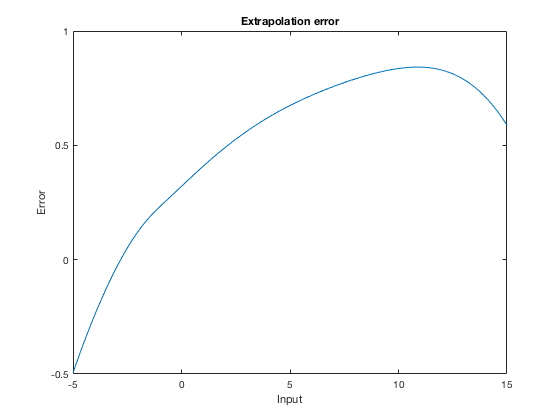
\includegraphics[width=0.4\textwidth]{extrap_error}
	\caption{Extrapolation error (in units of $\sigma$) \label{fig:extrap_error}}
\end{center}
\end{figure}
\end{centering}

In the case of the extrapolation error especially, few if any conclusions should be drawn. The dependence of the network on initial conditions and weights mean that these performance values cannot be assumed even for similar networks in similar conditions.

\section{Conclusions}
The ability of a simple, one layer neural network to model a non-linear function without noise was examined. It was determined that above a threshold value there was no significant improvement in network performance, with the risk of overfitting rising as the number of neurons increased. The network was determined to be successful at predicting interpolated values within the training domain to within the provided parameters for accuracy. An examination of the network's ability to extrapolate outside of the training domain was made, though conclusions should not be drawn from the performance of this precise network in this case due to the sensitivity of this method to the selection of initial conditions.

\end{document}